% Community edition maintained by Saleh Alqahtani (@smaq777).
% Substantially reorganised and extended from the publicly available
% UTS thesis template by Dr Chandranath Adak (LPPL 1.3c).
\documentclass[a4paper,12pt,openany,oneside]{memoir}

% Core packages for the community edition. Reusable typography and memoir styling
% live in config/visual-style.tex so students can change presentation independently
% from packages and thesis content.
\usepackage{fontspec}
\defaultfontfeatures{Ligatures=TeX}
\usepackage[english]{babel}
\usepackage{microtype}
\usepackage{graphicx}
\usepackage{calc}
\usepackage{soul}
\usepackage{tikz}
\usetikzlibrary{arrows.meta,positioning,shapes.geometric}
\usepackage{booktabs}
\usepackage{tabularx}
\usepackage{longtable}
\usepackage{threeparttable}
\usepackage{array}
\usepackage{amsmath,amssymb}
\usepackage{xcolor}
\usepackage{xparse}
\usepackage{xstring}
\usepackage[normalem]{ulem}
\usepackage{marginnote}
\usepackage{hyperref}
\usepackage[nameinlink,noabbrev]{cleveref}
\usepackage[round,authoryear]{natbib}

\hypersetup{
  colorlinks=true,
  linkcolor=black,
  citecolor=black,
  urlcolor=blue!55!black
}

\newcommand{\placeholder}[1]{\textcolor{gray!70!black}{\textit{[Replace this example: #1]}}}
\newcommand{\keywords}[1]{\par\noindent\textbf{Keywords:} #1}

% Public-safe visual system for the community template.
% This file contains presentation only: no thesis-specific structure or content.

% TeX Gyre Schola is a portable Schoolbook-style family bundled with current
% TeX Live and MiKTeX distributions.
\setmainfont{texgyreschola-regular.otf}[
  BoldFont=texgyreschola-bold.otf,
  ItalicFont=texgyreschola-italic.otf,
  BoldItalicFont=texgyreschola-bolditalic.otf
]
\setsansfont{texgyreheros-regular.otf}[
  BoldFont=texgyreheros-bold.otf,
  ItalicFont=texgyreheros-italic.otf,
  BoldItalicFont=texgyreheros-bolditalic.otf
]
\setmonofont{lmmono10-regular.otf}[ItalicFont=lmmono10-italic.otf]

\definecolor{ThesisGrey}{gray}{0.55}
\definecolor{ThesisRule}{gray}{0.18}

% A4 layout inspired by the maintained community edition's established memoir
% presentation. Change these values only after checking every output PDF.
\settrimmedsize{297mm}{210mm}{*}
\settypeblocksize{634pt}{*}{*}
\setulmargins{40mm}{*}{*}
\setlrmarginsandblock{26.5mm}{26.5mm}{*}
\setmarginnotes{17pt}{51pt}{\onelineskip}
\setheadfoot{30pt}{2\onelineskip}
\setheaderspaces{*}{2\onelineskip}{*}
\checkandfixthelayout
\OnehalfSpacing
\raggedbottom
\frenchspacing
\setlength{\emergencystretch}{2em}

% Standard hierarchy: chapters, sections and subsections are numbered. Students
% may add or remove headings; the table of contents is generated automatically.
\setsecnumdepth{subsection}
\maxsecnumdepth{subsubsection}
\maxtocdepth{subsection}

% Distinctive main-matter chapter opener: vertical CHAPTER label, large grey box,
% and a right-aligned title. It does not prescribe chapter names or chapter count.
\makeatletter
\newsavebox{\CommunityChapterBox}
\newcommand{\CommunityChapterMarker}[1][4cm]{%
  \sbox{\CommunityChapterBox}{%
    \resizebox{!}{#1}{\fboxsep=1pt%
      \colorbox{ThesisGrey}{\color{white}\thechapter}}}%
  \rotatebox{90}{%
    \resizebox{\heightof{\usebox{\CommunityChapterBox}}+
      \depthof{\usebox{\CommunityChapterBox}}}{!}{\scshape\so\@chapapp}}\quad
  \raisebox{\depthof{\usebox{\CommunityChapterBox}}}{\usebox{\CommunityChapterBox}}%
}
\newcommand{\CommunityChapterNumber}[1][4cm]{%
  \sbox{\CommunityChapterBox}{\CommunityChapterMarker[#1]}%
  \makebox[0pt][c]{\makebox[1cm][r]{\usebox{\CommunityChapterBox}}}%
}

\makechapterstyle{communitymain}{%
  \renewcommand\chapnamefont{\normalfont\Large\scshape\raggedleft\so}
  \renewcommand\chaptitlefont{\normalfont\Large\bfseries\scshape}
  \renewcommand\chapternamenum{}
  \renewcommand\printchaptername{}
  \renewcommand\printchapternum{\null\hfill\CommunityChapterNumber[2.5cm]\par}
  \renewcommand\afterchapternum{\par\vskip\midchapskip}
  \renewcommand\printchaptertitle[1]{%
    \color{ThesisGrey}\chaptitlefont\raggedleft ##1\par}
}

% Front matter uses the same restrained grey language without a numbered marker.
\makechapterstyle{communityfront}{%
  \renewcommand\chapnamefont{\normalfont\Large\scshape}
  \renewcommand\chaptitlefont{\normalfont\Large\bfseries\scshape}
  \renewcommand\printchaptername{}
  \renewcommand\printchapternum{}
  \renewcommand\afterchapternum{}
  \renewcommand\printchaptertitle[1]{%
    \centering\color{ThesisGrey}\chaptitlefont ##1\par}
  \setlength{\beforechapskip}{42pt}
  \setlength{\afterchapskip}{36pt}
}
\makeatother

% Continuation pages carry a restrained running chapter header and rule. Chapter
% opening and front-matter pages retain only the centred page number.
\makepagestyle{communitymain}
\makeoddfoot{communitymain}{}{\thepage}{}
\makeevenfoot{communitymain}{}{\thepage}{}
\makeheadrule{communitymain}{\textwidth}{\normalrulethickness}
\makeoddhead{communitymain}{}{}{\small\textsc{\leftmark}}
\makeevenhead{communitymain}{}{}{\small\textsc{\leftmark}}
\renewcommand*{\chaptermark}[1]{%
  \markboth{\chaptername\space\thechapter.\space #1}{}}

\makepagestyle{communityplain}
\makeoddfoot{communityplain}{}{\thepage}{}
\makeevenfoot{communityplain}{}{\thepage}{}
\makeoddhead{communityplain}{}{}{}
\makeevenhead{communityplain}{}{}{}
\aliaspagestyle{chapter}{communityplain}

% Declaration-page initial. The surrounding statement remains a placeholder and
% must always be replaced with the student's current official wording.
\newcommand{\DeclarationInitial}[1]{%
  \raisebox{-0.50\height}{%
    \fontsize{58}{58}\selectfont\bfseries\textcolor{ThesisGrey}{#1}}%
  \hspace{-0.18em}%
}

% Replace every value below with your own verified information.
\newcommand{\ThesisTitle}{An Example Research Thesis: Replace This with Your Approved Title}
\newcommand{\ThesisAuthor}{Student Name}
\newcommand{\StudentID}{00000000}
\newcommand{\DegreeName}{Doctor of Philosophy}
\newcommand{\SchoolName}{Your School}
\newcommand{\FacultyName}{Your Faculty}
\newcommand{\PrincipalSupervisor}{Principal Supervisor Name}
\newcommand{\CoSupervisor}{Co-supervisor Name}
\newcommand{\SubmissionMonth}{Month}
\newcommand{\SubmissionYear}{20XX}


% This community repository distributes no university logo.
% To use an authorised logo, add assets/institution-logo.pdf.
\newcommand{\InstitutionName}{Your University}
\newcommand{\InstitutionLogo}{%
  \IfFileExists{assets/institution-logo.pdf}{%
    \includegraphics[width=42mm]{assets/institution-logo.pdf}%
  }{%
    \fbox{\parbox[c][28mm][c]{60mm}{\centering\small
      Replace with your authorised\\institution logo\\or remove this box}}%
  }%
}


% Accessible colours from a colour-blind-friendly palette. IDs remain visible
% so meaning never depends on colour alone.
\definecolor{ExaminerOne}{HTML}{0072B2}
\definecolor{ExaminerTwo}{HTML}{D55E00}
\definecolor{ExaminerThree}{HTML}{CC79A7}
\definecolor{DeletedText}{HTML}{666666}

\newif\ifReviewCopy
\IfStrEq{\ThesisReviewMode}{review}{\ReviewCopytrue}{\ReviewCopyfalse}

\newcommand{\ApplyExaminerColour}[1]{%
  \IfBeginWith{#1}{E1}{\color{ExaminerOne}}{%
    \IfBeginWith{#1}{E2}{\color{ExaminerTwo}}{%
      \IfBeginWith{#1}{E3}{\color{ExaminerThree}}{\color{black}}}}}

\newcommand{\ExaminerBadge}[1]{%
  \begingroup\ApplyExaminerColour{#1}\textbf{[#1]}\endgroup}

% Usage: \CorrectionAdd{E1-01}{a}{new text}
\NewDocumentCommand{\CorrectionAdd}{m m m}{%
  \label{corr:#1-#2}%
  \ifReviewCopy
    \begingroup\ApplyExaminerColour{#1}\textbf{[#1]}~#3\endgroup%
    \marginnote{\ExaminerBadge{#1}}%
  \else
    #3%
  \fi}

% Usage: \CorrectionReplace{E2-03}{a}{old text}{new text}
\NewDocumentCommand{\CorrectionReplace}{m m m m}{%
  \label{corr:#1-#2}%
  \ifReviewCopy
    \begingroup\color{DeletedText}\sout{#3}\endgroup{}%
    \begingroup\ApplyExaminerColour{#1} \textbf{[#1]}~#4\endgroup%
    \marginnote{\ExaminerBadge{#1}}%
  \else
    #4%
  \fi}

% Usage: \CorrectionDelete{E1-05}{a}{text that was removed}
\NewDocumentCommand{\CorrectionDelete}{m m m}{%
  \label{corr:#1-#2}%
  \ifReviewCopy
    \begingroup\color{DeletedText}\textbf{[#1 deleted]}~\sout{#3}\endgroup%
    \marginnote{\ExaminerBadge{#1}}%
  \fi}


\hypersetup{pdftitle={\ThesisTitle},pdfauthor={\ThesisAuthor}}

\begin{document}
\frontmatter
\chapterstyle{communityfront}
\pagestyle{communityplain}
\begin{titlingpage}
\centering
\InstitutionLogo

\vspace{2cm}
{\Large\bfseries \ThesisTitle\par}
\vspace{1.5cm}
{\large \ThesisAuthor\par}
{\normalsize Student ID: \StudentID\par}

\vfill
A thesis submitted in fulfilment of the requirements for the degree of\\
\textbf{\DegreeName}

\vspace{1cm}
\SchoolName\\
\FacultyName\\
\InstitutionName

\vspace{1cm}
\SubmissionMonth{} \SubmissionYear
\end{titlingpage}


\cleardoublepage
\chapter*{Certificate of Original Authorship}
\addcontentsline{toc}{chapter}{Certificate of Original Authorship}

\placeholder{Insert the exact current authorship declaration required by your university.}

\vspace{2em}
I certify that this thesis is my own work except where properly acknowledged.
I understand that university wording and disclosure requirements may change,
including requirements concerning editorial assistance and generative AI.

\vspace{3em}
\noindent Signed: \rule{6cm}{0.4pt}\hfill Date: \rule{3cm}{0.4pt}


\cleardoublepage
\chapter*{Dedication}
\addcontentsline{toc}{chapter}{Dedication}
\begin{center}
\itshape
\placeholder{Write a short dedication, or remove this page.}
\end{center}


\cleardoublepage
\chapter*{Acknowledgements}
\addcontentsline{toc}{chapter}{Acknowledgements}

\placeholder{Thank supervisors, collaborators, participants, funders, family and
community members as appropriate. Check whether funding bodies require exact wording.}

Example: I sincerely thank my supervisory panel for their guidance throughout
this research. I am also grateful to the participants who generously contributed
their time and experience. Any remaining errors are my own.


\cleardoublepage
\chapter*{Abstract}
\addcontentsline{toc}{chapter}{Abstract}

\placeholder{Replace this example with a self-contained summary of the problem,
method, principal results, contribution and implications. Use verified numbers.}

Example structure: This thesis investigates a clearly defined research problem
within a specified context. It uses a transparent research design to collect and
analyse relevant evidence. The findings identify an important pattern and explain
its significance for theory and practice. The thesis contributes a reproducible
approach and identifies limitations that should guide future research.

\keywords{example keyword; research method; thesis template; replace these terms}


\cleardoublepage
\chapter*{Thesis Format}
\addcontentsline{toc}{chapter}{Thesis Format}

\placeholder{State whether the thesis is a conventional monograph, thesis by
publication, creative work with exegesis, or another approved format.}

Example: This thesis is presented as a conventional monograph. Chapters 1--3
establish the research problem and methodology, Chapters 4--5 report and discuss
the findings, and Chapter 6 presents the conclusions and recommendations.


\cleardoublepage
\chapter*{Publications and Presentations}
\addcontentsline{toc}{chapter}{Publications and Presentations}

\placeholder{List only verified outputs and explain how each relates to the thesis.}

Example:\begin{itemize}
  \item Student, A. and Supervisor, B. (20XX). ``Example publication title.''
  \emph{Example Journal}. Status: published / accepted / under review.
\end{itemize}


\cleardoublepage
\chapter*{Statement of Author Contributions}
\addcontentsline{toc}{chapter}{Statement of Author Contributions}

\placeholder{For thesis-by-publication content, state each contributor's role and
use the exact authorship requirements supplied by your school or university.}

Example: The student led the study design, data analysis and manuscript drafting.
The supervisory panel contributed methodological guidance, critical revision and
research oversight.


\cleardoublepage

\tableofcontents*
\cleardoublepage
\listoffigures
\cleardoublepage
\listoftables
\cleardoublepage
\chapter*{Abbreviations}
\addcontentsline{toc}{chapter}{Abbreviations}
\begin{description}
  \item[HDR] Higher Degree by Research
  \item[AI] Artificial Intelligence
  \item[UTS] University of Technology Sydney
\end{description}
\placeholder{Remove unused examples and add only abbreviations used in your thesis.}


\cleardoublepage

\mainmatter
\chapterstyle{communitymain}
\pagestyle{communitymain}
\chapter{Introduction}
\label{chap:introduction}

\placeholder{Rename this chapter and replace every example paragraph with your own work.}

\section{Background and context}
Start broadly enough for a reader outside your immediate specialisation. Define the
real-world or scholarly setting, introduce the central concepts, and support factual
claims with authoritative sources. For example, research projects often become harder
to maintain when their writing, evidence, figures and revision history are scattered
across unrelated files \citep{knuth1984texbook}.

\subsection{Moving from a broad setting to a precise focus}
A subsection develops one part of the chapter argument without creating a new chapter.
This fully synthetic example demonstrates the standard hierarchy automatically:
Chapter~1 contains Section~1.1, which contains Subsection~1.1.1. Students should use
headings only when they help a reader follow the logic of the real thesis.

\section{Problem statement and research gap}
State what is known, what remains unresolved, and why that unresolved issue matters.
Avoid presenting a broad topic as though it were automatically a research gap.

\CorrectionAdd{E1-01}{a}{Although prior work explains how structured authoring tools
support reproducible documents, there remains limited practical guidance connecting
large-thesis file organisation, transparent examiner revisions and multiple submission
outputs in one maintainable workflow. This thesis addresses that operational gap.}

\section{Aim, objectives and research questions}
The aim should describe the overall intellectual destination. Objectives are the
concrete steps used to reach it, while research questions define what the thesis will
answer. A student could adapt the following pattern:
\begin{quote}
\textbf{Aim:} To investigate how \placeholder{phenomenon} affects
\placeholder{population or system} in \placeholder{context}.
\end{quote}

\begin{enumerate}
  \item Review and synthesise the relevant literature.
  \item Design and apply an appropriate research method.
  \item Analyse the evidence and explain its implications.
\end{enumerate}

\begin{description}
  \item[RQ1] How does \placeholder{factor A} influence \placeholder{outcome B}?
  \item[RQ2] Under what conditions does that relationship change?
\end{description}

\section{Illustrative contributions}
\begin{table}[htbp]
  \centering
  \caption{Example contribution map}
  \label{tab:contribution-map}
  \begin{tabularx}{\textwidth}{@{}p{0.20\textwidth}XX@{}}
    \toprule
    \textbf{Contribution} & \textbf{Claim to be demonstrated} & \textbf{Evidence location} \\
    \midrule
    C1 & A clearly defined conceptual or empirical contribution. & \Cref{chap:literature,chap:results} \\
    C2 & A methodological or practical contribution. & \Cref{chap:methodology,chap:discussion} \\
    C3 & A set of implications grounded in the study evidence. & \Cref{chap:discussion,chap:conclusion} \\
    \bottomrule
  \end{tabularx}
\end{table}


Do not claim novelty merely because a technique is new to your project. Connect every
claimed contribution to evidence developed in later chapters.

\section{Thesis structure}
\Cref{chap:literature} synthesises prior research. \Cref{chap:methodology} explains the
research design, \Cref{chap:results} reports the evidence, and \Cref{chap:discussion}
interprets it. \Cref{chap:conclusion} answers the research questions and identifies
future work.

\chapter{Literature Review}
\label{chap:literature}

\section{Purpose and scope}
Explain what the review covers, its boundaries and how it supports the research
questions. A literature review should synthesise relationships and disagreements,
not become a sequence of disconnected paper summaries.

\section{Search and selection approach}
Report databases, search concepts, date ranges, inclusion criteria and the final
screening process at a level another researcher could understand. If the thesis is not
a formal systematic review, describe the approach accurately rather than adopting a
label that the method cannot support.

\section{Theme one: structured scholarly writing}
Structured source documents separate content from presentation and allow the same
material to be transformed consistently \citep{lamport1994latex}. The practical
value for a large thesis is not simply attractive typesetting: stable labels,
bibliographic automation and modular files reduce avoidable maintenance work.

\section{Theme two: transparent revision}
Revision evidence should connect a specific examiner comment to a specific substantive
change. Colour can assist navigation, but identifiers such as \texttt{E1-01} preserve
meaning when a document is printed in greyscale or read with assistive technology.

\section{Synthesis and conceptual framework}
Compare the themes, explain their relationship, and end with the precise proposition
or gap taken into the methodology. \Cref{tab:literature-synthesis} demonstrates a
compact synthesis table.

\begin{table}[htbp]
  \centering
  \caption{Example literature synthesis table}
  \label{tab:literature-synthesis}
  \newcolumntype{Y}{>{\raggedright\arraybackslash}X}
  \begin{tabularx}{\textwidth}{@{}>{\raggedright\arraybackslash}p{0.18\textwidth}YYY@{}}
    \toprule
    \textbf{Theme} & \textbf{What is established} & \textbf{What is contested or missing} & \textbf{Relevance to this thesis} \\
    \midrule
    Structured writing & Modular sources improve document maintainability. & Practical workflows vary across disciplines. & Motivates the file architecture. \\
    Revision evidence & Traceable responses improve review transparency. & Colour-only systems create accessibility risks. & Motivates IDs plus colour. \\
    \bottomrule
  \end{tabularx}
\end{table}


\chapter{Methodology}
\label{chap:methodology}

\section{Research design}
Name and justify the research design in relation to the research questions. Explain
why it is a better fit than plausible alternatives, and distinguish the overall
methodology from individual data-collection methods.

\section{Study workflow}
\begin{figure}[htbp]
  \centering
  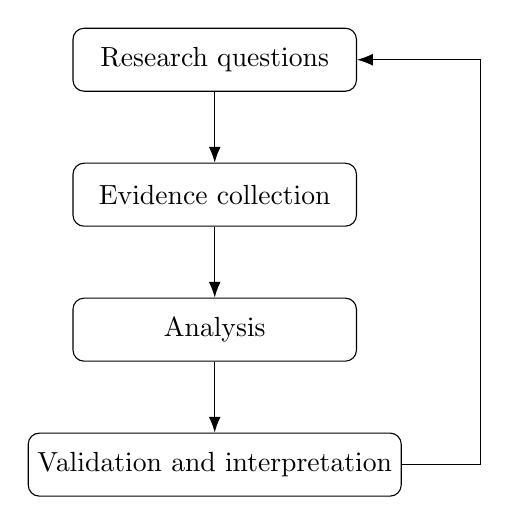
\begin{tikzpicture}[
  node distance=9mm,
  every node/.style={draw,rounded corners,align=center,minimum width=3.6cm,minimum height=8mm},
  every path/.style={draw,-{Latex[length=2mm]}}
]
  \node (questions) {Research questions};
  \node (evidence) [below=of questions] {Evidence collection};
  \node (analysis) [below=of evidence] {Analysis};
  \node (validation) [below=of analysis] {Validation and interpretation};
  \path (questions) -- (evidence);
  \path (evidence) -- (analysis);
  \path (analysis) -- (validation);
  \path (validation.east) -- ++(1.0,0) |- (questions.east);
\end{tikzpicture}


  \caption{Example research workflow drawn directly in \LaTeX.}
  \label{fig:research-workflow}
\end{figure}

\CorrectionAdd{E2-01}{a}{As illustrated in \Cref{fig:research-workflow}, the research
questions determine the evidence required, the analysis converts that evidence into
findings, and validation checks whether the resulting interpretation is sufficiently
supported. The arrows represent an iterative process rather than an irreversible
pipeline.}

\section{Data collection or evidence generation}
Describe who or what supplied the evidence, how items were selected, the procedure,
instrument quality and any departures from the approved protocol. Replace this example
with enough detail for a knowledgeable reader to assess validity and reproducibility.

\section{Analysis}
Define every measure and connect it to the question it answers. For example, an
illustrative normalised change can be expressed as
\begin{equation}
  \Delta_{i}=\frac{x_{i,\mathrm{post}}-x_{i,\mathrm{pre}}}{
  \max(x_{i,\mathrm{pre}},\epsilon)},
  \label{eq:normalised-change}
\end{equation}
where $x_{i,\mathrm{pre}}$ and $x_{i,\mathrm{post}}$ are the verified measurements for
case $i$, and $\epsilon>0$ prevents division by zero. Equation~\eqref{eq:normalised-change}
is an example only; students must use an analysis justified for their own evidence.

\section{Ethics, integrity and data management}
State the relevant approval identifier, consent arrangements, privacy safeguards,
storage and retention controls. Never copy an example approval number. Follow the
current instructions from your institution, faculty or school and research ethics
office.


\chapter{Results}
\label{chap:results}

\section{Chapter overview}
Report findings in the order needed to answer the research questions. Keep observation
separate from interpretation when that distinction helps the reader; the discussion
chapter can then explain meaning, implications and relationship to prior work.

\section{Example descriptive results}
The deliberately small dataset below shows how a student can combine a caption, stable
label, numeric alignment and an explanatory note without converting the table to an image.
\begin{table}[htbp]
  \centering
  \caption{Synthetic example results (replace completely)}
  \label{tab:sample-results}
  \begin{tabularx}{\textwidth}{@{}Xrrr@{}}
    \toprule
    \textbf{Group} & \textbf{$n$} & \textbf{Mean} & \textbf{SD} \\
    \midrule
    Example A & 24 & 4.20 & 0.61 \\
    Example B & 26 & 4.68 & 0.57 \\
    \bottomrule
  \end{tabularx}
  \par\smallskip
  \begin{minipage}{\textwidth}\footnotesize
    \textit{Note.} All values are invented solely to demonstrate table formatting.
  \end{minipage}
\end{table}


The synthetic values in \Cref{tab:sample-results} demonstrate formatting only. They do
not represent participants, experiments or findings from Saleh Alqahtani, UTS, Dr
Chandranath Adak or any other person or institution.

\section{Example analytical result}
A useful results paragraph identifies the comparison, reports the estimate and its
uncertainty, and then states the factual result without exaggerating what the design
can establish. Replace this paragraph with verified output from your own analysis.

\CorrectionAdd{E3-01}{a}{These illustrative results cannot support scientific or
institutional conclusions because the values are deliberately synthetic. In a real
thesis, the limitations must address sampling, measurement, analytical assumptions,
missing evidence and the boundaries of generalisation.}

\chapter{Discussion}
\label{chap:discussion}

\section{Overview of principal findings}
Begin by answering the research questions in plain academic language. Do not repeat
the entire results chapter; identify the most consequential findings and their
relationship to the thesis aim.

\section{Interpretation in relation to prior work}
Explain where the findings agree with, extend or challenge the literature reviewed in
\Cref{chap:literature}. Consider credible alternative explanations. A strong discussion
shows how the evidence supports the interpretation and where uncertainty remains.

\section{Theoretical and practical implications}
Separate implications that follow directly from the evidence from recommendations that
depend on additional assumptions. Identify the intended audience and the conditions
under which each implication is likely to apply.

\section{Strengths and limitations}
Discuss limitations precisely rather than adding a generic disclaimer. Explain their
likely direction or consequence, the mitigation used, and what remains unresolved.
Strengths should also be linked to specific design or evidence features.


\chapter{Conclusion}
\label{chap:conclusion}

\section{Research questions revisited}
Answer each research question directly using findings already established in the
thesis. The conclusion should not introduce a new dataset, method or major argument.

\section{Contributions}
Return to the claims in \Cref{tab:contribution-map} and state the demonstrated
contribution, its evidence and its boundary. Remove any contribution that the completed
study does not actually substantiate.

\section{Recommendations and future research}
Prioritise a small number of feasible recommendations. Future research should arise
from the study's limitations or new questions exposed by the findings, not from a
generic statement that more research is needed.

\section{Closing statement}
End with a concise statement of what the reader should remember. This final paragraph
is an opportunity to reconnect the technical contribution to the larger problem
introduced in \Cref{chap:introduction}.



\appendix
\chapter{Example Research Instrument}
\label{app:instrument}

\placeholder{Replace this appendix with material required to understand or audit your study.}

Appendices may contain instruments, supplementary derivations, extended tables,
technical specifications or other supporting evidence. Each appendix should be cited
from the main thesis and should not be used to hide material essential to the argument.

\section{Illustrative prompts}
\begin{enumerate}
  \item Describe \placeholder{the experience, process or observation}.
  \item What factors influenced \placeholder{the outcome of interest}?
  \item Is there anything else relevant to the research question?
\end{enumerate}



\backmatter
\bibliographystyle{plainnat}
\bibliography{bibliography/references}
\end{document}
